%----------------------------------------------------------------------------
\chapter{Monitor forráskód generátor}
%----------------------------------------------------------------------------

%----------------------------------------------------------------------------
\section{A monitor interfészei}
%----------------------------------------------------------------------------

A monitorozás alatt lévő rendszer egy közös interfészen keresztül kommunikál a monitorral. Az interfész Java implementációja a 19. ábrán tekinthető meg. A monitor azt vizsgálja, hogy a rendszer a scenario szerint működik-e.

Monitor interfész:
\begin{itemize}
    \item update(): a monitorban tárolt rendszer állapotát frissíti a paraméterben kapott üzenet alapján.
    \item goodStateReached(): a rendszer aktuális állapotát jelzi.
    \item requirementSatisfied(): jelzi hogy a rendszer megfelel-e a követelménynek
    \item errorDetected(): detektált hiba jelzésére szolgál
\end{itemize}

Az update() függvényt a rendszer hívja, hogy továbbítsa az üzenetet a monitornak. Paraméterként az üzenet küldőjét (sender), fogadóját (receiver), üzenet nevét (messageType) és az üzenet paramétereit várja (parameters). A goodStateReached() függvényt a monitor hívja amikor a rendszer állapota változik. Ha a rendszer nem elfogadó állapotban van akkor igazat ad vissza, ha pedig nem akkor hamisat. A requirementSatisfied() függvényt is a monitor hívja. Ha a követelménynek megfelelt a rendszer viselkedése akkor igazat ad vissza, amúgy hamisat.

Az üzenetek megfigyeléséhez szükséges segédfüggvényeket a kommunikációs infrastruktúrához kézzel kell megírni. Ezek a monitort az update() függvényen keresztül hívják.

\begin{lstlisting}[language=java,frame=single, float=h!, caption={Monitor interfész Java implementációja.},captionpos=b]
public interface IMonitor {
	public boolean goodStateReached();
	public void update(String sender, String receiver, String messageType, String[] parameters);
	public boolean requirementSatisfied();
	public void errorDetected(String sender, String receiver, String messageType, String[] parameters);
}
\end{lstlisting}

Az időzitő komponenshez tartozik egy időzitő interfész amin keresztül elérhető a komponens. Ezen az interfészen keresztül lehet az óraváltozokat lekérdezni vagy nullázni. Két függvénye van:
\begin{itemize}
    \item getClock(String clock): óraváltozó lekérdezése név alapján
    \item resetClock(String clock): óraváltozó nullázása név alapján
\end{itemize}

\begin{lstlisting}[language=java,frame=single, float=h!, caption={Időzitő interfész Java implementációja.},captionpos=b]
public interface IClock {
	public long getClock(String clock);
	public void resetClock(String clock);
}
\end{lstlisting}

%----------------------------------------------------------------------------
\section{A monitor forráskód megvalósítása}
%----------------------------------------------------------------------------
A generált forráskód struktúrája egy statikus és egy dinamikus részből áll.
A statikus részbe az időzitett automata java osztályai kerülnek:
\begin{itemize}
    \item State: egy állapotot leíró osztály
    \item Transition: egy élet reprezentáló osztály
    \item Automaton: egy automatát megvalósitó osztály
\end{itemize}

A monitor interfész, a monitor java osztálya, az időzítő interfész és a hozzá tartozó java osztály is ebbe a részbe tartozik.

A dinamikus részben található a Specification Java osztály, ami a scenario alapján generált automata forráskódját tartalmazza. Ezt a 20. ábra mutatja be. A dinamikus rész pirosan van bekeretezve és a statikus rész pedig feketén.

\begin{figure}[!ht]
    \centering
    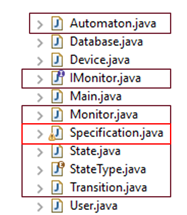
\includegraphics[width=150mm, keepaspectratio]{figures/18abra.png}
    \caption{A monitor forráskódjának struktúrája.}
\end{figure}

A szükséges forráskódok generálásához az Xtend technológiát használtam. Az előző fejezetben ismertetett generátort kiegészítettem egy Monitor Java osztállyal, ami a monitor forráskódjának implementációját tartalmazza.

%----------------------------------------------------------------------------
\section{Minta példa}
%----------------------------------------------------------------------------

A 21. ábrán látható egy scenario követelmény, amit egy példa okos telefon működésére specifikáltunk. Az okos telefonon van egy zene lejátszási lista generáló alkalmazás. A követelményben azt várjuk el, hogy ha a felhasználó megnyitja az alkalmazást akkor a belső kamera készít az arcáról egy képet. A kép alapján eldönti, hogy milyen a felhasználó kedve és az alapján előállít egy zene lejátszási listát.

A 23. ábrán látható az okos telefon és a monitor közti kapcsolat megvalósítása Java kódban és a 22. ábrán pedig egy monitor kimenet. A monitor a rendszertől kapott üzenetek alapján jelzi, hogy a követelmény alapján mi a rendszer állapota.

\begin{lstlisting}[frame=single, float=ht!, caption={Okos telefon működésére megadott scenario követelmény.},captionpos=b]
specification spec1 {
	object User user;
	object Device device;
	object Database db;

	constraint error {
		message closeApp() user -> device;
	}

	scenario playlist_generation{
		message openApp() user -> device;
		message accessWebcam() device -> device;
		message getPhoto() required device -> user;
		message cameraOffline() fail user -> device;
		message retrieveMood() required strict device -> db;
		message retrieveMusic() required device -> db;
		message generatePlaylist() strict db -> device;
	}
}
\end{lstlisting}

\begin{lstlisting}[frame=single, float=ht!, caption={Generált automata Never claim formátumba.},captionpos=b]
never{ /*playlist_generationMonitor*/
T0_init:
 if
 :: (!(user.openApp().device)) -> goto T0_init
 :: (user.openApp().device) -> goto T0_q1
 fi;
T0_q1:
 if
 :: (!(device.accessWebcam().device)) -> goto T0_q1
 :: (device.accessWebcam().device) -> goto T0_q2
 fi;
T0_q2:
 if
 :: (!(device.getPhoto().user)) -> goto T0_q2
 :: (!(device.getPhoto().user)) -> goto accept_q3
 :: (device.getPhoto().user) -> goto T0_q4
 fi;
accept_q3:
 if
 fi;
T0_q4:
 if
 :: (!(user.cameraOffline().device)) -> goto T0_q6
 :: (!(user.cameraOffline().device)) -> goto T0_q4
 :: (user.cameraOffline().device) -> goto accept_q5
 fi;
accept_q5:
 if
 fi;
T0_q6:
 if
 :: (device.retrieveMood().db) -> goto T0_q8
 :: (!(device.retrieveMood().db)) -> goto accept_q7
 fi;
accept_q7:
 if
 fi;
T0_q8:
 if
 :: (!(device.retrieveMusic().db)) -> goto T0_q8
 :: (!(device.retrieveMusic().db)) -> goto accept_q9
 :: (device.retrieveMusic().db) -> goto T0_q10
 fi;
accept_q9:
 if
 fi;
T0_q10:
 if
 :: (db.generatePlaylist().device) -> goto T0_q11
 fi;
T0_q11:
 if
 fi;
}
\end{lstlisting}

\begin{lstlisting}[language=java, frame=single, float=ht!, caption={Az okos telefon és hozzá tartozó monitor összecsatolásának Java implementációja.},captionpos=b]
public class Main {
	public static void monitorStatus(String status) {
		System.out.println(status);
	}

	public static void main(String[] args) {
		Specification specification = new Specification();
		specification.listAutomatas();
		IMonitor monitor = new Monitor(specification.getAutomata().get(0));

		User user = new User();
		Device device = new Device();
		Database db = new Database();
		user.device = device;
		device.user = user;
		device.db = db;
		db.device = device;
		user.monitor = monitor;
		device.monitor = monitor;
		db.monitor = monitor;

		user.init();
	}
}
\end{lstlisting}

\begin{lstlisting}[language=java, frame=single, float=ht!, caption={Az okos telefon Java osztálya.},captionpos=b]
public class Device {
	public IMonitor monitor;
	public User user;
	public Database db;

	void openApp() {
		monitor.update("user", "device", "openApp", new String[] {});
		accessWebcam();
	}

	void accessWebcam() {
		monitor.update("device", "device", "accessWebcam", new String[] {});
		user.getPhoto();
		db.retrieveMood();
		db.retrieveMusic();
	}

	void cameraOffline() {
		monitor.update("user", "device", "cameOffline", new String[] {});
	}

	void generatePlaylist() {
		monitor.update("db", "device", "generatePlaylist", new String[] {});
	}
}
\end{lstlisting}

A 24. ábrán látható az okos telefon Java osztálya. Megtekinthető a monitor és az eszköz közti kommunikáció megvalósítása is.

\begin{figure}[!ht]
    \centering
    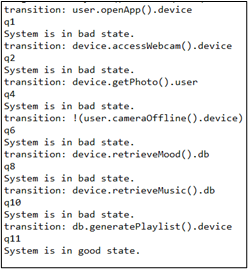
\includegraphics[width=150mm, keepaspectratio]{figures/23abra.png}
    \caption{Monitor kimenete a rendszer működésének egyes fázisaiban.}
\end{figure}
A 25. ábrán látszik, hogy a rendszer a működése elején nem felelt meg a monitor követelményének. Amikor a működése végére ért akkor a monitor jelezte, hogy a követelmény teljesült a „Good state” üzenettel. A mintához tartozó Specification osztály a függelékben található. A generált automatát a konstruktorában állítja elő.

%----------------------------------------------------------------------------
\section{Összetett szerkezetek}
%----------------------------------------------------------------------------

A monitor forráskód generátor támogatja az alt, par vagy loop operátorokat tartalmazó scenariokat is. Erre példát a függelékben lehet találni.

%----------------------------------------------------------------------------
\section{Időzítési feltételek}
%----------------------------------------------------------------------------

A monitor forráskód generátor támogatja az időzítési feltételeket tartalmazó scenariokat is.